\documentclass[11pt,aspectratio=169]{beamer}

\usetheme{metropolis}
\usecolortheme{default}
\metroset{numbering=fraction, progressbar=frametitle, sectionpage=none}

\setbeamertemplate{navigation symbols}{}
\setbeamercolor{frametitle}{bg=mDarkTeal, fg=white}
\setbeamercolor{progress bar}{fg=mDarkTeal, bg=mDarkTeal!20}
\definecolor{mDarkTeal}{HTML}{23373B}
\definecolor{mAccent}{HTML}{EB811B}

\usepackage{amsmath,amssymb}
\usepackage{graphicx}
\usepackage{booktabs}
\usepackage{appendixnumberbeamer}
\usepackage{tikz}
\usepackage{wasysym}

\title{Math Bootcamp}
\subtitle{Day 1 --- Foundations (Sections 1.1--1.9)}
\author{Math Camp 2026}
\date{}

\newcommand{\QFrame}[1]{%
  \begin{frame}{#1 \quad {\small\textcolor{mAccent}{Together}}}}

\begin{document}

\begin{frame}
  \titlepage
\end{frame}

\section{1.1 --- Notation and Number Systems}

\begin{frame}{1.1 Number systems --- names and definitions}
  \small
  \begin{tabular}{@{}clp{0.48\textwidth}@{}}
    \toprule
    \textbf{Symbol} & \textbf{English name} & \textbf{What it is} \\
    \midrule
    $\mathbb{N}$ & natural numbers & Non-negative integers for \textbf{counting} \\
    $\mathbb{Z}$ & integers & $\ldots,-2,-1,0,1,2,\ldots$ \\
    $\mathbb{Q}$ & rational numbers & Fractions $p/q$ ($q\ne0$) \\
    $\mathbb{R}$ & real numbers & All points on the number line \\
    $\mathbb{R}^n$ & $n$-dimensional real space & Lists / vectors of length $n$ \\
    \bottomrule
  \end{tabular}

  \medskip
  \begin{center}
  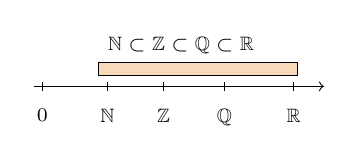
\begin{tikzpicture}[scale=0.55, every node/.style={font=\scriptsize}]
    \draw[->] (-0.2,0) -- (6.5,0);
    \foreach \x/\lab in {0/0,1.5/$\mathbb{N}$,2.8/$\mathbb{Z}$,4.2/$\mathbb{Q}$,5.8/$\mathbb{R}$}
      \draw (\x,0.1) -- (\x,-0.1) node[below=3pt] {\lab};
    \draw[fill=mAccent!30] (1.3,0.25) rectangle (5.9,0.55);
    \node at (3.2,0.95) {$\mathbb{N}\subset\mathbb{Z}\subset\mathbb{Q}\subset\mathbb{R}$};
  \end{tikzpicture}
  \end{center}
\end{frame}

\begin{frame}{1.1 Symbols and vectors --- names and definitions}
  \textbf{Common symbols}
  \small
  \begin{tabular}{@{}cl@{\quad}cl@{}}
    $\in$ & ``is an element of'' &
    $\forall$ & ``for all'' \\
    $\exists$ & ``there exists'' &
    $\Rightarrow$ & ``implies'' \\
    & &
    $\Leftrightarrow$ & ``if and only if'' (iff) \\
  \end{tabular}

  \medskip
  \normalsize
  \textbf{Scalar vs.\ vector}
  \small
  \begin{itemize}
    \item \textbf{Scalar:} one number, e.g.\ income $w\in\mathbb{R}$
    \item \textbf{Vector:} a list of numbers
      $\mathbf{x}=(x_1,\ldots,x_n)\in\mathbb{R}^n$
    \item \textbf{Dot product:} $\mathbf{p}\cdot\mathbf{x}=\sum_{i=1}^n p_i x_i$
  \end{itemize}
\end{frame}

\QFrame{1.1 --- Which set?}
  \small
  \textbf{Smallest set that fits?}

  \medskip
  \onslide<2->{\textbf{1.} The number of girlfriends / boyfriends you can have\par}
  \onslide<3->{\textcolor{mAccent}{$\rightarrow\;\mathbb{N}$}\hfill
    {\scriptsize counting: $0,1,2,\ldots$}\par\medskip}

  \onslide<4->{\textbf{2.} Money you spend at a vending machine (e.g.\ HK\$8.50)\par}
  \onslide<5->{\textcolor{mAccent}{$\rightarrow\;\mathbb{Q}$}\hfill
    {\scriptsize e.g.\ $8.50=17/2$ dollars}\par\medskip}

  \onslide<6->{\textbf{3.} Order as a vector: (HK\$ spent on drink, \# snacks) = $(8.50,\,2)$\par}
  \onslide<7->{\textcolor{mAccent}{$\rightarrow\;(8.50,\,2)\in\mathbb{Q}\times\mathbb{N}$}\par}
\end{frame}

\section{1.2 --- Logic and Mathematical Statements}

\begin{frame}{1.2 Logic --- names and definitions}
  \footnotesize
  \begin{tabular}{@{}llp{0.52\textwidth}@{}}
    \toprule
    \textbf{English} & \textbf{Symbol} & \textbf{Meaning} \\
    \midrule
    $P$ \textbf{only if} $Q$ & $P\Rightarrow Q$ &
      $Q$ is \textbf{necessary} for $P$ (without $Q$, no $P$) \\[4pt]
    $P$ \textbf{if} $Q$ & $Q\Rightarrow P$ &
      $Q$ is \textbf{sufficient} for $P$ ($Q$ alone is enough) \\[4pt]
    $P$ \textbf{if and only if} $Q$ & $P\Leftrightarrow Q$ &
      $Q$ is necessary \textbf{and} sufficient \\[4pt]
    \textbf{Contrapositive} & $\neg Q\Rightarrow\neg P$ &
      same truth as $P\Rightarrow Q$:\\
    & & if $Q$ fails, $P$ must fail \\
    \bottomrule
  \end{tabular}
\end{frame}

\QFrame{1.1 --- IKEA run}
  \footnotesize
  \textbf{First week in HK:} you go to IKEA and spot three plush toys.

  \medskip
  \begin{columns}[T,onlytextwidth]
    \column{0.32\textwidth}
    \centering
    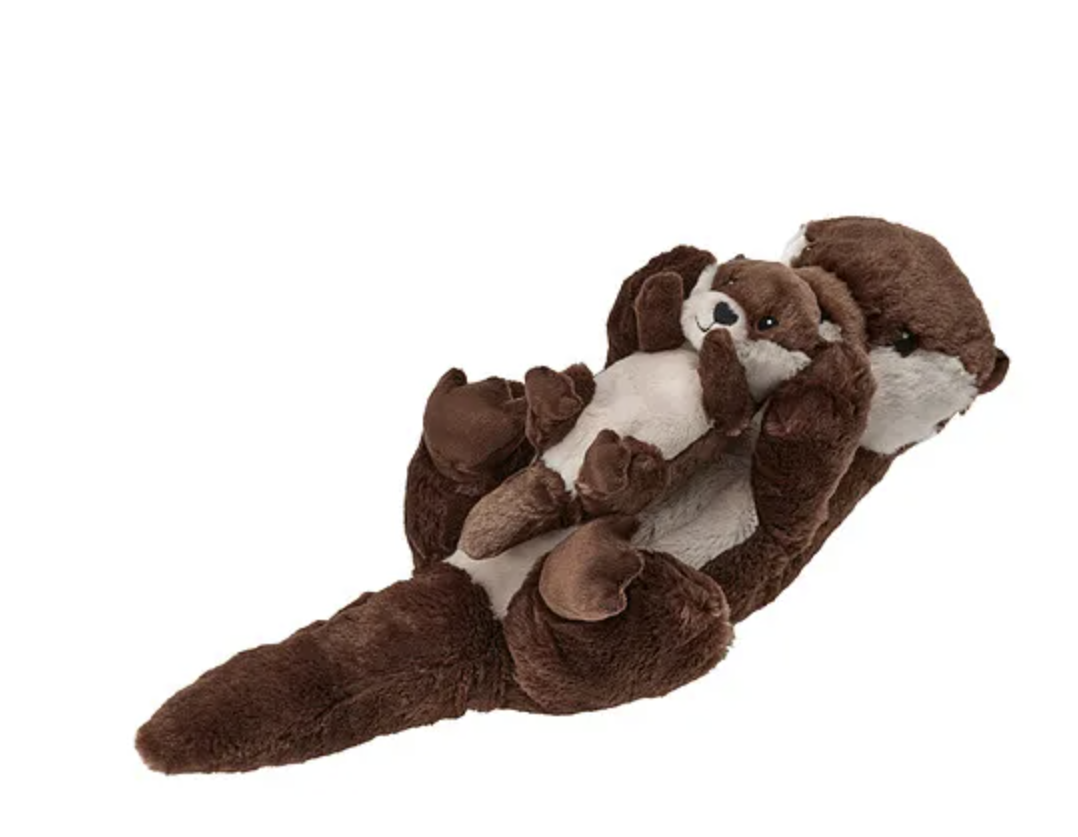
\includegraphics[width=\linewidth]{figures/otter.png}\\[2pt]
    Otter \quad HK\$179.9

    \column{0.32\textwidth}
    \centering
    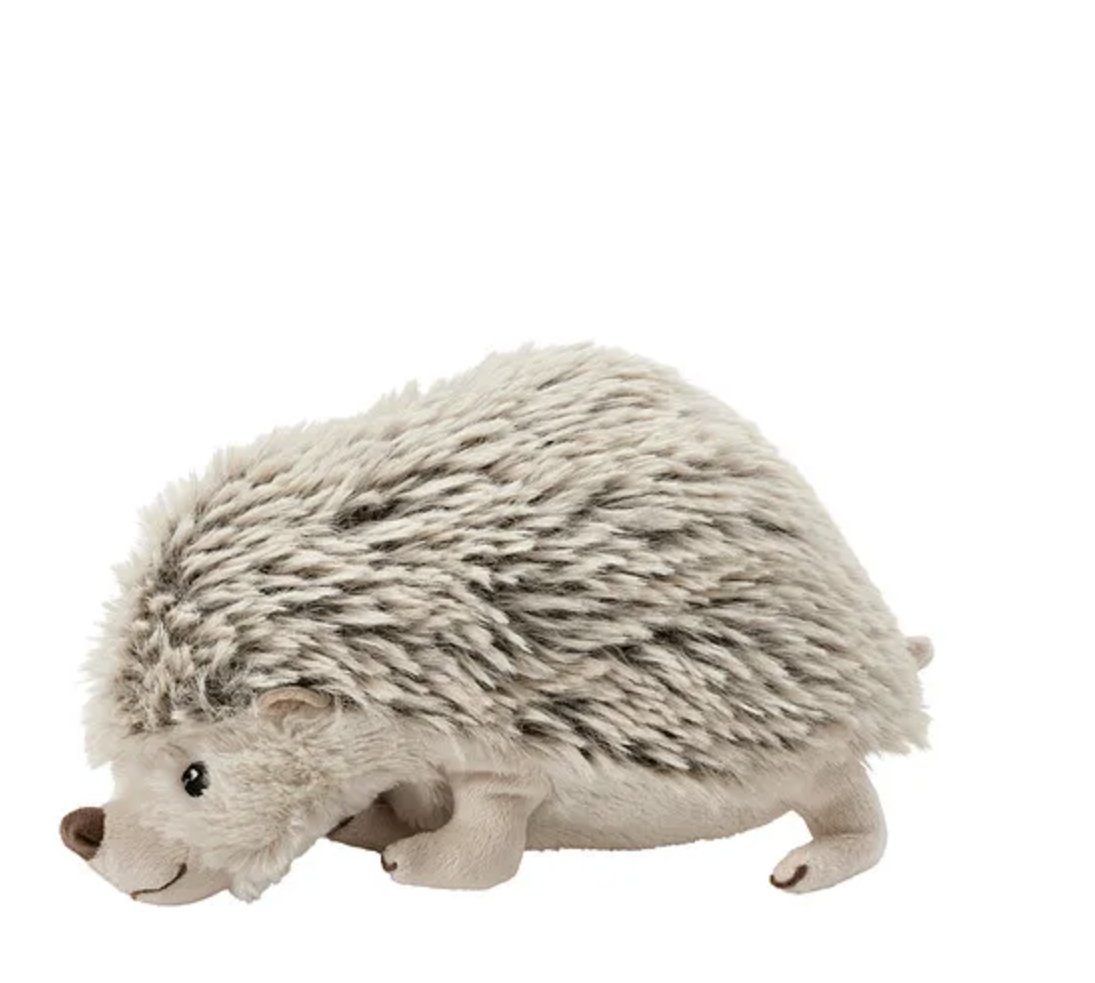
\includegraphics[width=\linewidth]{figures/hedgehog.png}\\[2pt]
    Hedgehog \quad HK\$79.9

    \column{0.32\textwidth}
    \centering
    
\includegraphics[width=\linewidth]{figures/shark.jpg}\\[2pt]
    BLÅHAJ \quad HK\$179.9
  \end{columns}

  \medskip
  You have \textbf{HK\$500} pocket money ($B=500$).

  \medskip
  Basket $\mathbf{x}\in\mathbb{N}^3$: \# otters, \# hedgehogs, \# sharks.
  E.g.\ $(1,\,1,\,0)$ = one otter, one hedgehog, no shark.
  Price vector $\mathbf{p}=(179.9,\,79.9,\,179.9)\in\mathbb{Q}^3$.
  Budget set:
  $\mathcal{B}=\{\mathbf{x}\in\mathbb{N}^3:\mathbf{p}\cdot\mathbf{x}\le 500\}$.
\end{frame}

\QFrame{1.2 --- Plush symbols practice}
  \scriptsize
  $\mathbf{p}=(179.9,\,79.9,\,179.9)$,\ $\mathcal{B}=\{\mathbf{x}\in\mathbb{N}^3:\mathbf{p}\cdot\mathbf{x}\le 500\}$.
  \textbf{True or false?}

  \vspace{2pt}
  \onslide<2->{\textbf{1.} [$\in$]\ $(0,0,3)\in\mathcal{B}$}\;
  \onslide<3->{\textcolor{mAccent}{\textbf{False}} {\tiny ($539.7>500$)}}\par
  \onslide<4->{\textbf{2.} [$\subset$]\ $\mathbb{N}^3\subset\mathcal{B}$}\;
  \onslide<5->{\textcolor{mAccent}{\textbf{False}} {\tiny (e.g.\ $(3,0,0)\notin\mathcal{B}$)}}\par
  \onslide<6->{\textbf{3.} [$\forall$]\ $\forall\,\mathbf{x}\in\mathcal{B},\;\mathbf{x}\ne(0,1,0)$}\;
  \onslide<7->{\textcolor{mAccent}{\textbf{False}} {\tiny ($(0,1,0)\in\mathcal{B}$)}}\par
  \onslide<8->{\textbf{4.} [$\exists$]\ $\exists\,\mathbf{x}\in\mathcal{B},\;\mathbf{x}=(3,0,0)$}\;
  \onslide<9->{\textcolor{mAccent}{\textbf{False}} {\tiny ($539.7>500$)}}\par
  \onslide<10->{\textbf{5.} [$\Rightarrow$]\ $(1,1,1)\in\mathcal{B}$ \textbf{only if}
    $\mathbf{p}\cdot(1,1,1)\le 500$}\;
  \onslide<11->{\textcolor{mAccent}{\textbf{True}} {\tiny ($439.7\le 500$)}}\par
  \onslide<12->{\hspace{1.5em}{\tiny also True: $(1,1,1)\in\mathcal{B}$ \textbf{if}
    $\mathbf{p}\cdot(1,1,1)\le 500$}}\par
  \onslide<13->{\textbf{6.} [$\Rightarrow$]\ $(0,0,3)\in\mathcal{B}$ \textbf{if}
    $(1,1,1)\in\mathcal{B}$}\;
  \onslide<14->{\textcolor{mAccent}{\textbf{False}} {\tiny ($(1,1,1)\in\mathcal{B}$ but $539.7>500$)}}\par
  \onslide<15->{\textbf{7.} [contrapositive]\ If
    $\mathbf{p}\cdot(1,1,1)+\mathbf{p}\cdot(0,1,0)>500$, then
    $(1,1,1)\notin\mathcal{B}$ \textbf{or} $(0,1,0)\notin\mathcal{B}$}\;
  \onslide<16->{\textcolor{mAccent}{\textbf{False}} {\tiny ($519.6>500$, yet each basket alone is in $\mathcal{B}$)}}\par
  \onslide<17->{\hspace{1.5em}{\tiny each affordable $\not\Rightarrow$ jointly affordable}}\par
\end{frame}

\section{1.3 --- Sets and Set Operations}

\begin{frame}{1.3 Sets and operations --- names and definitions}
  \scriptsize
  \begin{tabular}{@{}clp{0.38\textwidth}@{}}
    \toprule
    \textbf{Symbol} & \textbf{Name} & \textbf{Meaning} \\
    \midrule
    $\in$, $\notin$ & element / not in & $x$ belongs (or not) to $A$ \\
    $\subset$, $=$ & subset, equality & $A\subset B$; $A=B$ iff mutual $\subset$ \\
    $\emptyset$, $\{\,\}$, $\{x\in S:\ldots\}$ & sets & empty, roster, set-builder \\
    $A\cup B$, $A\cap B$ & union, intersection & in $A$ or $B$; in both \\
    $A^c$, $A\setminus B$ & complement, difference & not in $A$; in $A$ not $B$ \\
    $A\times B$ & Cartesian product & pairs $(a,b)$, $a\in A$, $b\in B$ \\
    \bottomrule
  \end{tabular}

  \medskip
  \textbf{In economics:}\quad
  budget set $\mathcal{B}\subset\mathbb{N}^3$;\;
  $(8.50,\,2)\in\mathbb{Q}\times\mathbb{N}$.
\end{frame}

\QFrame{1.3 --- Set operations (IKEA)}
  \scriptsize
  $\mathcal{B}=\{\mathbf{x}\in\mathbb{N}^3:\mathbf{p}\cdot\mathbf{x}\le 500\}$,\quad
  $\mathcal{H}=\{\mathbf{x}\in\mathbb{N}^3:\text{middle entry}\ge 1\}$ (at least one hedgehog).

  \vspace{2pt}
  \textbf{Describe the set.}

  \vspace{2pt}
  \onslide<2->{\textbf{1.} $\mathcal{B}\cap\mathcal{H}$}\;
  \onslide<3->{\textcolor{mAccent}{affordable baskets with $\ge 1$ hedgehog}
    {\tiny (e.g.\ $(0,1,0)$)}}\par
  \onslide<4->{\textbf{2.} $\mathcal{B}\cup\mathcal{H}$}\;
  \onslide<5->{\textcolor{mAccent}{affordable baskets \textbf{or} baskets with $\ge 1$ hedgehog}}\par
  \onslide<6->{\textbf{3.} $\mathcal{B}\setminus\mathcal{H}$}\;
  \onslide<7->{\textcolor{mAccent}{affordable baskets with \textbf{no} hedgehog}
    {\tiny (e.g.\ $(1,0,0)$)}}\par
  \onslide<8->{\textbf{4.} $(179.9,\,79.9)\in\mathbb{Q}\times\mathbb{Q}$ but
    $(179.9,\,79.9)\notin\mathcal{B}$}\;
  \onslide<9->{\textcolor{mAccent}{True}\;
    {\tiny Cartesian product $\ne$ budget set --- pairs $\ne$ baskets}}\par
  \onslide<10->{\textbf{5.} $(1,0,0)\subset\mathcal{B}$}\;
  \onslide<11->{\textcolor{mAccent}{\textbf{False}}\;
    {\tiny $(1,0,0)$ is a basket: use $(1,0,0)\in\mathcal{B}$ (True);
    but $\{(1,0,0)\}\subset\mathcal{B}$ is True}}\par
\end{frame}

\section{1.4 --- Functions}

\begin{frame}{1.4 Functions --- names and definitions}
  \scriptsize
  \begin{tabular}{@{}clp{0.40\textwidth}@{}}
    \toprule
    \textbf{Term} & \textbf{Notation} & \textbf{Meaning} \\
    \midrule
    Function & $f\colon A\to B$ & each $x\in A$ maps to \textbf{exactly one} $f(x)\in B$ \\
    Domain & $A$ & allowed inputs \\
    Codomain & $B$ & target set --- every output must lie in $B$ \\
    Range & $f(A)$ & outputs hit: $\{f(x):x\in A\}\subseteq B$ \\
    Injective (one-to-one) &  & $f(x_1)=f(x_2)\Rightarrow x_1=x_2$ \\
    Surjective (onto) &  & every $y\in B$ equals some $f(x)$ \\
    Operations & $(f\pm g)(x)$, $(cf)(x)$, $(fg)(x)$ &
      $(f\pm g)(x)=f(x)\pm g(x)$;\ $(cf)(x)=c\,f(x)$;\ $(fg)(x)=f(x)g(x)$ \\
    Composition & $(f\circ g)(x)$ & apply $g$ first: $(f\circ g)(x)=f(g(x))$ \\
    \bottomrule
  \end{tabular}
\end{frame}

\QFrame{1.4 --- Ages}
  \small
  Define $f\colon D\to C$ by: $f(x)$ = your girlfriend / boyfriend's age
  when \textbf{your age} is $x$.

  \vspace{4pt}
  \onslide<2->{\textbf{1.} Domain $D$?}\;
  \onslide<3->{\textcolor{mAccent}{$\{22,23,\ldots,30\}$}\hfill
    {\scriptsize typical ages in a master's program}}\par
  \onslide<4->{\textbf{2.} Codomain $C$?}\;
  \onslide<5->{\textcolor{mAccent}{$\{18,19,\ldots,120\}$}\hfill
    {\scriptsize plausible partner ages}}\par
  \onslide<6->{\textbf{3.} Is $80\in f(D)$?}\;
  \onslide<7->{\textcolor{mAccent}{\textbf{Probably not}}\hfill
    {\scriptsize ($80\in C$, but $f(D)\subseteq\{17,\ldots,35\}$)}}\par
  \onslide<8->{\textbf{4.} Range $f(D)$?}\;
  \onslide<9->{\textcolor{mAccent}{your age $\pm 5$ on $D$}\hfill
    {\scriptsize $\{17,18,\ldots,35\}$}}\par
  \onslide<10->{\textbf{5.} Is $f$ surjective (onto $C$)?}\;
  \onslide<11->{\textcolor{mAccent}{\textbf{No}}\hfill
    {\scriptsize ($f(D)\ne C$; e.g.\ $120\in C$ but $120\notin f(D)$)}}\par
  \onslide<12->{\textbf{6.} Is $f$ injective (one-to-one)?}\;
  \onslide<13->{\textcolor{mAccent}{\textbf{Probably not}}\hfill
    {\scriptsize (e.g.\ $f(22)=f(30)=22$)}}\par
  \onslide<14->{\textbf{7.} If $f(25)=\{22,\,80\}$, is $f$ a function?}\;
  \onslide<15->{\textcolor{mAccent}{\textbf{No --- a correspondence}}\hfill
    {\scriptsize (a function gives \textbf{exactly one} output per input;
    it's immoral to have a correspondence\ \smiley)}}\par
\end{frame}

\section{1.5 --- Supremum and Infimum}

\QFrame{1.5 --- Reservation price (example first)}
  \small
  BLÅHAJ sticker price: \textbf{HK\$179.9}.
  You buy \textbf{only on sale}: when $p<179.9$.

  \medskip
  Prices where you still buy:
  $P=\{p\in\mathbb{R}_+:p<179.9\}$.

  \vspace{4pt}
  \onslide<2->{\textbf{Highest sale price you would accept?}}\;
  \onslide<3->{\textcolor{mAccent}{\textbf{No maximum in $P$}}\hfill
    {\scriptsize ($179.89$ works; so does $179.899$; \ldots)}}\par
  \onslide<4->{\textbf{Reservation price (WTP)?}}\;
  \onslide<5->{\textcolor{mAccent}{$\sup P=179.9$}\hfill
    {\scriptsize least upper bound --- the choke price)}}\par
  \onslide<6->{\textbf{Is $179.9\in P$?}}\;
  \onslide<7->{\textcolor{mAccent}{\textbf{No}}\hfill
    {\scriptsize at sticker price you walk away $\Rightarrow$ no $\max P$)}}\par
\end{frame}

\begin{frame}{1.5 Supremum and infimum --- names and definitions}
  \scriptsize
  \begin{tabular}{@{}clp{0.40\textwidth}@{}}
    \toprule
    \textbf{Term} & \textbf{Notation} & \textbf{Meaning} \\
    \midrule
    Maximum & $\max S$ & largest element \textbf{in} $S$ \\
    Minimum & $\min S$ & smallest element \textbf{in} $S$ \\
    Supremum & $\sup S$ & \textbf{least upper bound} of $S$ \\
    Infimum & $\inf S$ & \textbf{greatest lower bound} of $S$ \\
    \bottomrule
  \end{tabular}

  \medskip
  \textbf{Example (least upper bound):}\quad
  $S=[0,1)$.\ Upper bounds include $1,2,3,\ldots$;
  $\sup S=1$ --- the \textbf{smallest} upper bound ($1\notin S$).

  \medskip
  \textbf{Relations:}\quad
  if $\max S$ exists, $\max S=\sup S$;\ if $\min S$ exists, $\min S=\inf S$.

  \smallskip
  \hspace{2.1em}Always: $\inf S\le x\le\sup S$ for all $x\in S$.
\end{frame}

\section{1.6 --- Algebra Revision}

\begin{frame}{1.6 Taylor, logs, and exponentials}
  \scriptsize
  \textbf{Taylor expansion} (around $a$):
  \[
    f(a+h)=\sum_{k=0}^{\infty}\frac{f^{(k)}(a)}{k!}\,h^k
    =f(a)+f'(a)h+\frac{f''(a)}{2!}h^2+\frac{f^{(3)}(a)}{3!}h^3+\cdots
  \]

  \medskip
  \begin{tabular}{@{}ll@{\quad}ll@{}}
    \textbf{Logs} & & \textbf{Exponentials} & \\
    $\ln(ab)=\ln a+\ln b$ & & $e^{a+b}=e^a e^b$ & \\
    $\ln(x^\alpha)=\alpha\ln x$ & & $e^{\alpha x}=(e^x)^\alpha$ & \\
    $\ln(1+x)=x-\dfrac{x^2}{2}+\dfrac{x^3}{3}-\cdots$ & & $e^x=1+x+\dfrac{x^2}{2!}+\cdots$ & \\
  \end{tabular}

  \medskip
  \textbf{Quick check:}\quad
  $\ln(x_1^\alpha x_2^\beta)=\alpha\ln x_1+\beta\ln x_2$;\quad
  if $u=x_1^\alpha x_2^{1-\alpha}$, then
  $\ln u=\alpha\ln x_1+(1-\alpha)\ln x_2$.
\end{frame}

\begin{frame}{1.6 Why logs?}
  \small
  \begin{itemize}
    \item \textbf{Taylor:}\quad
      $f(a+h)\approx f(a)+f'(a)h$.
    \item \textbf{Apply to logs:}\quad
      $\ln(1+x)\approx x$ for small $x$.
    \item \textbf{Percentage changes:}\quad
      $\ln(x+\Delta x)-\ln x=\ln\!\bigl(1+\tfrac{\Delta x}{x}\bigr)\approx \tfrac{\Delta x}{x}$,
      so $\Delta\ln x$ tracks \textbf{\% change} in $x$.
    \item \textbf{Example:}\quad
      $\tfrac{\Delta x}{x}=5\%\Rightarrow \Delta\ln x\approx 0.05$.
    \item \textbf{Log--log regression:}\quad
      $\ln y=\alpha+\beta\ln x$.
    \item 1\% $\uparrow$ in $x$ $\Rightarrow$ $\beta$\% change in $y$.
    \item \textbf{Elasticity:}\quad
      $\varepsilon_{y,x}=\dfrac{\partial y}{\partial x}\dfrac{x}{y}
      =\dfrac{\Delta y/y}{\Delta x/x}
      =\dfrac{\partial\ln y}{\partial\ln x}$;\quad
      in $\ln y=\alpha+\beta\ln x$, $\varepsilon_{y,x}=\beta$.
  \end{itemize}
\end{frame}

\begin{frame}{1.6 Cobb--Douglas --- definition}
  \small
  \textbf{Utility / production:}
  \[
    U(x_1,x_2)=x_1^{\alpha}x_2^{1-\alpha},\qquad
    Y(K,L)=A K^{\alpha}L^{1-\alpha},\quad \alpha\in(0,1).
  \]

  \medskip
  \textbf{In logs (linear):}\quad
  $\ln U=\alpha\ln x_1+(1-\alpha)\ln x_2$;\quad
  $\ln Y=\ln A+\alpha\ln K+(1-\alpha)\ln L$.

  \medskip
  \textbf{Constant elasticity:}
  $\varepsilon_{U,x_1}=\dfrac{\partial\ln U}{\partial\ln x_1}=\alpha$,\quad
  $\varepsilon_{U,x_2}=1-\alpha$;\quad
  $\varepsilon_{Y,K}=\alpha$,\ $\varepsilon_{Y,L}=1-\alpha$.
  {\scriptsize Same numbers at every $(x_1,x_2)$ or $(K,L)$.}
\end{frame}

\begin{frame}{1.6 Why Cobb--Douglas? --- first-order approximation}
  \small
  \textbf{Any smooth utility $u(x_1,x_2)>0$:}\quad
  define $f(\ln x_1,\ln x_2)=\ln u(x_1,x_2)$.

  \medskip
  \textbf{First-order Taylor} around $(\ln\bar x_1,\ln\bar x_2)$:
  \[
    \ln u(x_1,x_2)
    \approx
    f(\ln\bar x_1,\ln\bar x_2)
    +\frac{\partial f}{\partial\ln x_1}\Big|_{\bar{\mathbf{x}}}(\ln x_1-\ln\bar x_1)
    +\frac{\partial f}{\partial\ln x_2}\Big|_{\bar{\mathbf{x}}}(\ln x_2-\ln\bar x_2).
  \]

  \medskip
  Let $\alpha_i=\dfrac{\partial\ln u}{\partial\ln x_i}\Big|_{\bar{\mathbf{x}}}$
  and absorb constants into $c$:
  \[
    \ln u(x_1,x_2)\approx c+\alpha_1\ln x_1+\alpha_2\ln x_2
    \quad\Leftrightarrow\quad
    u(x_1,x_2)\approx e^c\,x_1^{\alpha_1}x_2^{\alpha_2}.
  \]

  \medskip
  {\scriptsize Near $\bar{\mathbf{x}}$ only; Cobb--Douglas is exact when $\ln u$ is globally affine in logs.}
\end{frame}

\begin{frame}{1.6 Cobb--Douglas --- homogeneity and CRS}
  \scriptsize
  \textbf{Homogeneous of degree $k$:}\quad
  $f(t\mathbf{x})=t^k f(\mathbf{x})$ for $t>0$.

  \medskip
  \textbf{Utility}\ $U=x_1^{\alpha}x_2^{1-\alpha}$:\quad
  $U(tx_1,tx_2)=t^{\alpha}t^{1-\alpha}U(\mathbf{x})=t\,U(\mathbf{x})$
  $\Rightarrow$ degree~$1$.

  \medskip
  \textbf{Production}\ $Y=A K^{\alpha}L^{1-\alpha}$:\quad
  $Y(tK,tL)=t^{\alpha}t^{1-\alpha}Y(K,L)=t\,Y(K,L)$.

  \medskip
  \textbf{CRS (constant returns to scale):}\quad
  double all inputs $\Rightarrow$ double output (homogeneous of degree~$1$).
\end{frame}

\begin{frame}{1.6 Cobb--Douglas --- constant expenditure shares}
  \scriptsize
  Max $U=x_1^{\alpha}x_2^{1-\alpha}$ s.t.\ $p_1x_1+p_2x_2=w$.

  \medskip
  \textbf{FOC}\ (marginal utility per dollar equal):
  $\dfrac{\partial U/\partial x_1}{\partial U/\partial x_2}=\dfrac{p_1}{p_2}
  \Rightarrow \dfrac{\alpha/x_1}{(1-\alpha)/x_2}=\dfrac{p_1}{p_2}
  \Rightarrow \dfrac{p_1x_1}{p_2x_2}=\dfrac{\alpha}{1-\alpha}$.

  \medskip
  \textbf{Budget binds:}\ $p_1x_1+p_2x_2=w$.
  Substitute $p_1x_1=\dfrac{\alpha}{1-\alpha}\,p_2x_2$:
  \[
    w=p_2x_2\Bigl(\frac{\alpha}{1-\alpha}+1\Bigr)=\frac{p_2x_2}{1-\alpha}
    \Rightarrow p_2x_2=(1-\alpha)w,\quad p_1x_1=\alpha w.
  \]

  \medskip
  \textbf{Expenditure shares:}\ $\dfrac{p_1x_1}{w}=\alpha$,
  $\dfrac{p_2x_2}{w}=1-\alpha$ (constant).
\end{frame}

\begin{frame}{1.6 Why Cobb--Douglas? --- summary}
  \small
  \textbf{Why economists use Cobb--Douglas:}
  \begin{itemize}
    \item \textbf{Logs = \% changes:}\quad
      elasticities are $\partial\ln y/\partial\ln x$.
    \item \textbf{Local approximation:}\quad
      any smooth $u>0$ satisfies
      $\ln u\approx c+\alpha_1\ln x_1+\alpha_2\ln x_2$ near $\bar{\mathbf{x}}$.
    \item \textbf{Constant elasticity / shares:}\quad
      $\varepsilon_{u,x_i}=\alpha_i$; CD demands give fixed budget shares.
    \item \textbf{Homogeneity (degree~$1$) / CRS:}\quad
      $f(t\mathbf{x})=t f(\mathbf{x})$; double inputs $\Rightarrow$ double output.
    \item \textbf{Easy algebra:}\quad
      linear in logs, powers in levels; closed-form demands and FOCs.
    \item \textbf{Global use = modeling choice:}\quad
      tractability and homogeneity, not a theorem for all preferences.
  \end{itemize}
\end{frame}

\section{1.7 --- Single-Variable Derivatives}

\begin{frame}{1.7 Single-variable derivative --- formal definition}
  \small
  \textbf{Scope:}\ one independent variable.
  Partial derivatives ($\partial f/\partial x_i$) come later.

  \medskip
  \textbf{Definition.}\ For $f\colon\mathbb{R}\to\mathbb{R}$ and $a\in\mathbb{R}$,
  the \textbf{derivative at $a$} is
  \[
    f'(a)=\lim_{h\to 0}\frac{f(a+h)-f(a)}{h},
  \]
  provided the limit exists.
  Same number as $\dfrac{df}{dx}\Big|_{x=a}$.

  \medskip
  \textbf{Meaning:}\ instantaneous rate of change; slope of the tangent at $(a,f(a))$.

  \medskip
  {\scriptsize In economics: $MC=C'(q)$,\ $MU=U'(x)$,\ $MP_K=Y'(K)$.}
\end{frame}

\begin{frame}{1.7 Single-variable rules --- summary}
  \small
  \textbf{Single-variable calculus:}\ all rules below are for $f(x)$,
  $g(x)$, etc.
  Built from
  $f'(a)=\displaystyle\lim_{h\to 0}\frac{f(a+h)-f(a)}{h}$
  {\scriptsize (derivations in appendix)}:

  \medskip
  \footnotesize
  \begin{tabular}{@{}ll@{}}
    $(c)'=0$ &
    constant \\
    $(f\pm g)'=f'\pm g'$ &
    sum / difference \\
    $(x^n)'=nx^{n-1}$ &
    power rule \\
    $(fg)'=f'g+fg'$ &
    product rule \\
    $\Bigl(\tfrac{f}{g}\Bigr)'=\dfrac{f'g-fg'}{g^2}$ &
    quotient rule \\
    $(e^x)'=e^x$,\ $(\ln x)'=\tfrac{1}{x}$ &
    exp / log \\
    $(a^x)'=a^x\ln a$ &
    general exponential ($a>0$) \\
    $(f^{-1})'(y)=\dfrac{1}{f'(f^{-1}(y))}$ &
    inverse function \\
  \end{tabular}

  \medskip
  \textbf{Chain rule}\ (composition): if $y=f(u)$, $u=g(x)$, then
  $\dfrac{dy}{dx}=\dfrac{dy}{du}\cdot\dfrac{du}{dx}$.
\end{frame}

\begin{frame}{1.7 Single-variable chain rule}
  \small
  \textbf{Chain rule:}\ if $y=f(u)$ and $u=g(x)$, then
  \[
    \frac{dy}{dx}=\frac{dy}{du}\cdot\frac{du}{dx}
    =(f'\circ g)(x)\,g'(x).
  \]

  \medskip
  \textbf{Example:}\ $y=(3x+1)^5$.\ Let $u=3x+1$:
  $\dfrac{dy}{dx}=5u^4\cdot 3=15(3x+1)^4$.
\end{frame}

\QFrame{1.7 --- Single-variable marginals (Together)}
  \scriptsize
  \textbf{Differentiate}\ (one variable at a time).

  \vspace{4pt}
  \textbf{1.}\ Cubic cost:\ $C(q)=q^3-6q^2+15q+100$.
  \textcolor{mAccent}{$C'(q)=3q^2-12q+15$}\hfill
  {\tiny MC}\par\medskip

  \textbf{2.}\ Monopolist:\ $p(q)=120-2q$,\ $C(q)=q^2+10q+50$.
  Profit $\pi(q)=q(120-2q)-C(q)=110q-3q^2-50$.
  \textcolor{mAccent}{$\pi'(q)=110-6q$}\hfill
  {\tiny FOC: $q^*=110/6\approx18.3$}\par\medskip

  \textbf{3.}\ Cobb--Douglas production:\ $Y(K)=3K^{0.6}$.
  \textcolor{mAccent}{$Y'(K)=1.8\,K^{-0.4}$}\hfill
  {\tiny $MP_K$}\par\medskip

  \textbf{4.}\ Fixed cost + composite cost:\ $TC(q)=100+20(2q+1)^3$.
  \textcolor{mAccent}{$TC'(q)=120(2q+1)^2$}\hfill
  {\tiny chain rule}
\end{frame}

\begin{frame}{1.7 Euler's theorem}
  \vspace{-0.15cm}
  \footnotesize
  \setlength{\abovedisplayskip}{5pt}
  \setlength{\belowdisplayskip}{5pt}
  \textbf{Setup (from 1.6).}\ $f\colon\mathbb{R}^n\to\mathbb{R}$ is $C^1$,
  homogeneous of degree~$k$:\ $f(t\mathbf{x})=t^k f(\mathbf{x})$ for $t>0$.

  \smallskip
  \textbf{Euler's theorem.}\ $\displaystyle\sum_{i=1}^n x_i\,\frac{\partial f}{\partial x_i}(\mathbf{x})
    = k\,f(\mathbf{x})$.

  \smallskip
  \textbf{Proof.}\ Fix $\mathbf{x}$, $\varphi(t)=f(t\mathbf{x})=t^k f(\mathbf{x})$.

  \textbf{RHS:}\ $\varphi'(t)=k\,t^{k-1}f(\mathbf{x})$.\quad
  \textbf{LHS (chain rule):}\
  $\varphi'(t)=\sum_{i=1}^n \frac{\partial f}{\partial x_i}(t\mathbf{x})\,x_i$.

  At $t=1$:\ $\sum_i x_i f_{x_i}(\mathbf{x})=k f(\mathbf{x})$.

  \smallskip
  {\scriptsize Multivariate chain rule; partials defined formally in 1.8.}
\end{frame}

\begin{frame}{1.7 Euler's theorem --- the adding-up problem}
  \footnotesize
  \textbf{Economic question.}\ In a competitive economy, if labor and capital
  are each paid its \textbf{marginal product}, do total factor payments
  exactly equal total output? Or is there surplus profit or a deficit?

  \medskip
  This is the \textbf{adding-up problem} (Clark, Wicksteed).
  If payments do not exhaust output, marginal productivity theory of
  distribution looks inconsistent.

  \medskip
  \textbf{Mathematical condition.}\ Production $Q=f(K,L)$, CRS (degree~$1$):
  $f(tK,tL)=t\,f(K,L)$ for $t>0$.
  Euler's theorem ($k=1$):
  \[
    Q=\frac{\partial Q}{\partial K}\,K+\frac{\partial Q}{\partial L}\,L
    =MP_K\cdot K+MP_L\cdot L.
  \]
  {\scriptsize Algebra only so far --- no claim yet about wages or rents.}
\end{frame}

\begin{frame}{1.7 Euler's theorem --- competitive factor markets}
  \footnotesize
  \textbf{Total factor payments:}\ $rK+wL$.

  \medskip
  \textbf{Perfect competition in factor markets}\ $\Rightarrow$ each factor is
  paid its \textbf{value marginal product}:
  \[
    r=P\frac{\partial Q}{\partial K},\qquad
    w=P\frac{\partial Q}{\partial L}.
  \]

  \medskip
  \textbf{Euler (CRS, $k=1$).}\ $Q=\dfrac{\partial Q}{\partial K}K+\dfrac{\partial Q}{\partial L}L$.
  Multiply by $P$:
  \[
    PQ=rK+wL.
  \]
  Revenue equals factor payments --- output \textbf{exactly exhausted}; zero profit.

  \medskip
  {\scriptsize If returns to scale $\neq 1$, see IRS/DRS next.}
\end{frame}

\begin{frame}{1.7 Euler's theorem --- IRS and DRS}
  \footnotesize
  \textbf{CRS ($k=1$).}\ $PQ=rK+wL$ --- payments exhaust revenue; zero profit.

  \medskip
  \textbf{IRS ($k>1$).}\ Paying each factor its marginal product would cost
  \textbf{more} than revenue --- positive profit wedge (or inconsistency with
  perfect competition).

  \medskip
  \textbf{DRS ($k<1$).}\ MP payments \textbf{fall short} of revenue --- output
  not fully exhausted; surplus remains.

  \medskip
  {\scriptsize Intuition: under IRS, marginal contributions add up to more than
  current output; under DRS, to less.}
\end{frame}

\begin{frame}{1.7 Euler's theorem --- why IRS implies losses}
  \footnotesize
  \textbf{Better technology, IRS.}\ Production has \textbf{synergy} among inputs:
  at a given scale, doubling all inputs more than doubles output --- the extra
  is synergy.

  \medskip
  \textbf{Marginal product traps synergy.}\ $MP_K=\partial Q/\partial K$ holds
  $L$ (and other inputs) \textbf{fixed} at current levels.
  Those inputs are already in place, so an extra unit of $K$ gets credit for
  synergy between the new capital and existing labor.

  \medskip
  Repeat for every machine and every worker: the \textbf{same synergy} is
  credited to each input.
  Summing $MP_K\cdot K+MP_L\cdot L$ therefore \textbf{counts synergy several
  times}.

  \medskip
  \textbf{Euler.}\ Under IRS ($k>1$), $MP_K\cdot K+MP_L\cdot L=k\,Q>Q$.
  If each factor is paid its MP, total payments exceed revenue --- the firm
  would run \textbf{losses} under perfect competition.
\end{frame}

\section{1.8 --- Multivariate Calculus}

\begin{frame}{1.8 Level curves}
  \footnotesize
  \begin{columns}[T,onlytextwidth]
    \column{0.46\textwidth}
    \textbf{Multivariate function:}\ $z=f(x,y)$,\ e.g.\ utility $U(x_1,x_2)$.

    \medskip
    \textbf{Level curve} at height $c$:
    \[
      \mathcal{L}_c=\{(x,y)\in\mathbb{R}^2:f(x,y)=c\}.
    \]
    On a hill/mountain graph, slice the surface by the horizontal plane
    $z=c$; the slice projects to a level curve in the $(x,y)$-plane.

    \medskip
    \textbf{Contour map:}\ top-down picture of several $\mathcal{L}_c$'s.
    Along a level curve, $f$ is \textbf{constant}.

    \column{0.50\textwidth}
    \centering
    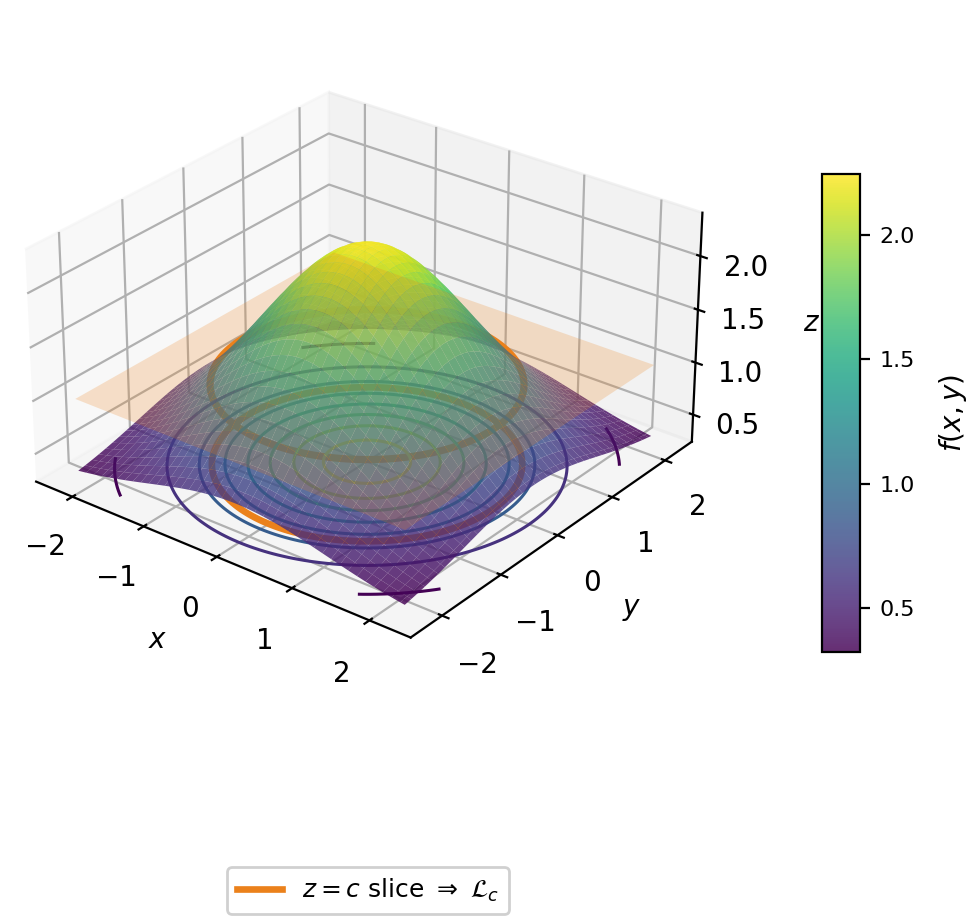
\includegraphics[width=\linewidth]{figures/level_surface_3d.png}
  \end{columns}
\end{frame}

\begin{frame}{1.8 Multivariate calculus --- roadmap}
  \small
  \textbf{Question:}\ how does $f(x,y)$ change when inputs move?
  \begin{itemize}
    \item Hold one variable fixed $\Rightarrow$ \textbf{partial derivatives}
    \item Small joint change $(dx,dy)$ $\Rightarrow$
      \textbf{total differential}
    \item Move in a chosen direction $\mathbf{u}$ $\Rightarrow$
      \textbf{directional derivative} (rate version of $df$)
    \item Differentiate in two orders $\Rightarrow$ \textbf{cross-partials}
      (Schwarz)
  \end{itemize}

\end{frame}

\begin{frame}{1.8 Partial derivatives}
  \footnotesize
  \begin{columns}[T,onlytextwidth]
    \column{0.50\textwidth}
    \textbf{Definition.}\ For $f(x,y)$,
    \[
      \frac{\partial f}{\partial x}(a,b)
      =\lim_{h\to 0}\frac{f(a+h,b)-f(a,b)}{h},
    \]
    holding $y=b$ fixed (and analogously $\partial f/\partial y$).

    \medskip
    \textbf{On a contour map:}\ fix $y=\bar y$ (horizontal line).
    The slope along that line is $\partial f/\partial x$.

    \medskip
    {\scriptsize Econ: $MP_K=\partial Y/\partial K$ with $L$ fixed.}

    \column{0.46\textwidth}
    \centering
    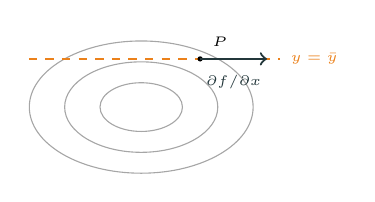
\begin{tikzpicture}[scale=0.68, every node/.style={font=\tiny}]
      \foreach \k in {0.7,1.3,1.9}
        \draw[gray!70] (0,0) ellipse ({\k*1.1} and {\k*0.65});
      \draw[dashed, mAccent, thick] (-2.1,0.9) -- (2.6,0.9)
        node[right] {$y=\bar y$};
      \fill (1.1,0.9) circle (1.4pt)
        node[above right=1pt] {$P$};
      \draw[thick, mDarkTeal, ->] (1.1,0.9) -- (2.35,0.9)
        node[midway, below=2pt] {$\partial f/\partial x$};
    \end{tikzpicture}
  \end{columns}
\end{frame}

\begin{frame}{1.8 Total differential}
  \vspace{-0.15cm}
  \small
  \setlength{\abovedisplayskip}{6pt}
  \setlength{\belowdisplayskip}{6pt}
  \textbf{Goal:}\ approximate how $f$ changes when $(x,y)$ moves a little
  from $(x_0,y_0)$ by $(\Delta x,\Delta y)$.

  \vspace{0.2cm}
  \setlength{\itemsep}{7pt}
  \begin{enumerate}
    \item \textbf{Exact change.}
      $\Delta z=f(x_0+\Delta x,y_0+\Delta y)-f(x_0,y_0)$.

    \item \textbf{Add/subtract} at $(x_0+\Delta x,y_0)$:
      \[
        \Delta z=
        \bigl[f(x_0+\Delta x,y_0+\Delta y)-f(x_0+\Delta x,y_0)\bigr]
        +\bigl[f(x_0+\Delta x,y_0)-f(x_0,y_0)\bigr].
      \]

    \item \textbf{Mean value theorem} ($\theta_1,\theta_2\in(0,1)$):
      \[
        \begin{aligned}
          f(x_0+\Delta x,y_0+\Delta y)-f(x_0+\Delta x,y_0)
          &=f_y(x_0+\Delta x,y_0+\theta_1\Delta y)\,\Delta y,\\
          f(x_0+\Delta x,y_0)-f(x_0,y_0)
          &=f_x(x_0+\theta_2\Delta x,y_0)\,\Delta x.
        \end{aligned}
      \]

    \item \textbf{Small steps} $\Delta x,\Delta y\to 0$:
      $\Delta z\approx f_x\,\Delta x+f_y\,\Delta y=:dz$,
      \quad $\nabla f=(f_x,f_y)$.
  \end{enumerate}
\end{frame}

\begin{frame}[plain]{}
  \centering
  \vspace{-0.2cm}
  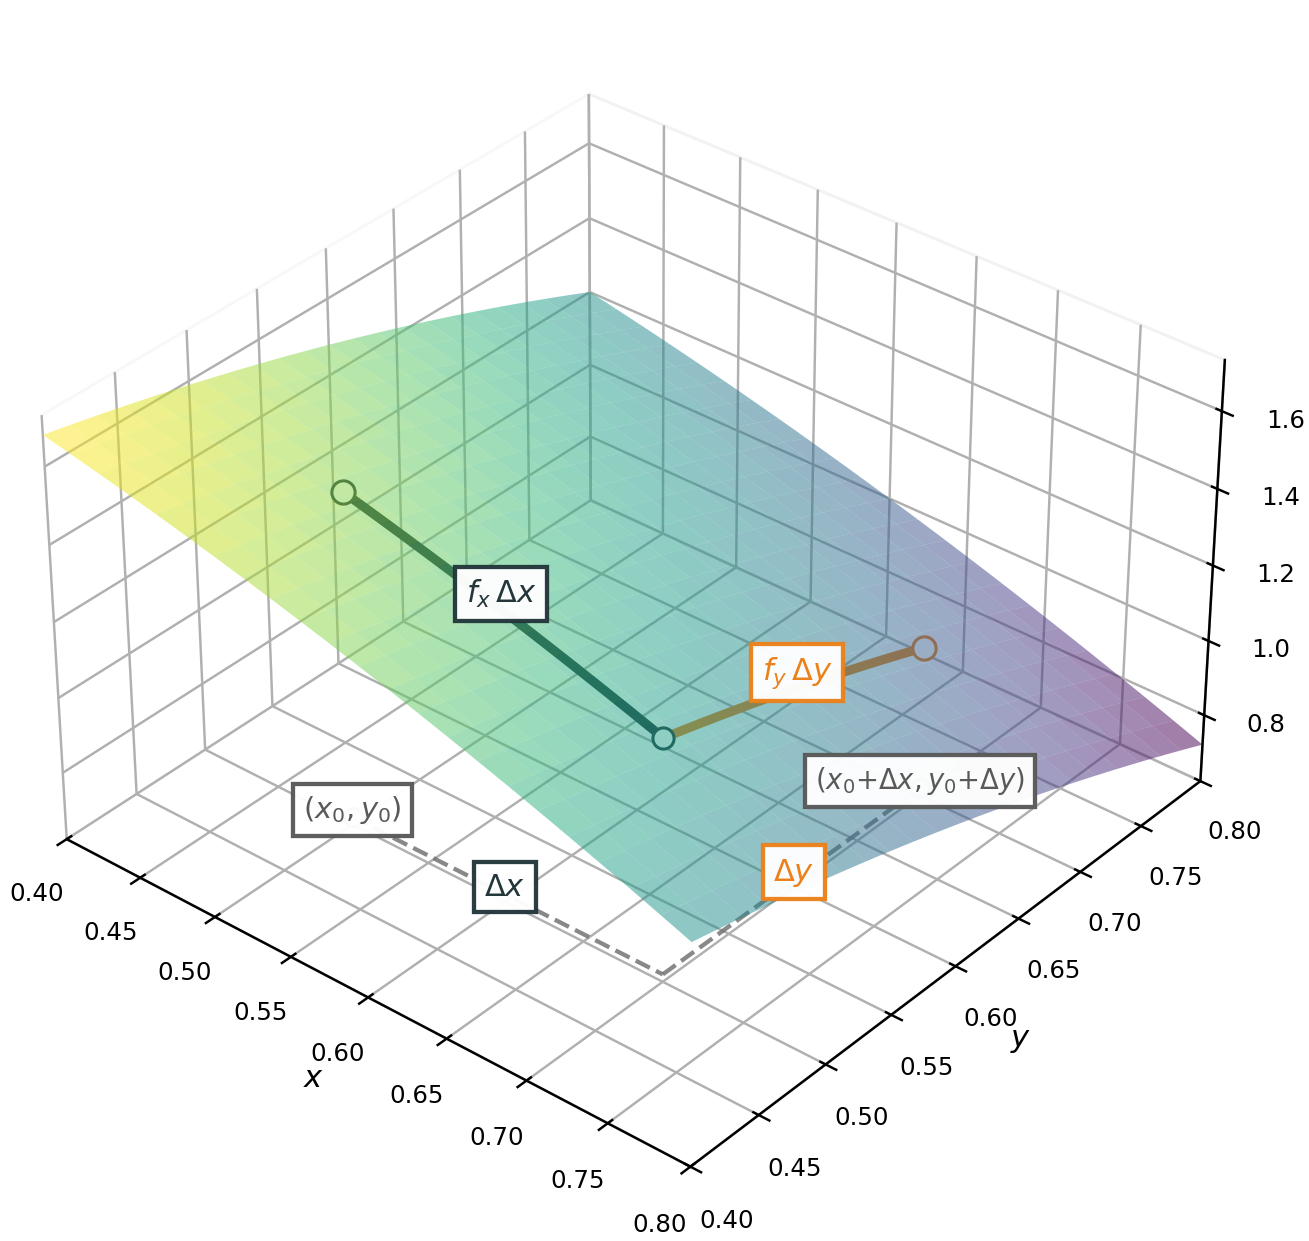
\includegraphics[height=0.96\textheight,keepaspectratio]{figures/total_differential_3d.png}
\end{frame}

\begin{frame}{1.8 Using the total differential}
  \footnotesize
  \textbf{When:}\ approximate how output changes when \textbf{several inputs}
  move a little (comparative statics, linearization).

  \medskip
  \textbf{Example.}\ Cobb--Douglas production
  $Y=3K^{\alpha}L^{1-\alpha}$ with $\alpha=0.5$, at $(K_0,L_0)=(100,64)$,
  $dK=2$, $dL=1$:
  \[
    dY=\underbrace{1.5K^{-0.5}L^{0.5}}_{MP_K}\,dK
       +\underbrace{1.5K^{0.5}L^{-0.5}}_{MP_L}\,dL.
  \]
  \[
    dY=\frac{1.5}{10}\cdot 8\cdot 2+\frac{1.5\cdot 10}{8}\cdot 1
    =2.4+1.875\approx 4.28.
  \]
  Exact: $Y(100,64)=240$,\ $Y(102,65)=3\sqrt{6630}\approx 244.27$,
  so $\Delta Y\approx 4.27$ (close to $dY$ when $dK,dL$ are small).
\end{frame}

\begin{frame}{1.8 Gradient and level curves}
  \vspace{-0.25cm}
  \begin{columns}[T,onlytextwidth]
    \column{0.40\textwidth}
    \scriptsize
    \textbf{At $P$ on $\mathcal{L}_c$:\quad}
    $\nabla f(P)\perp\mathcal{L}_c$ and points \textbf{uphill}.

    \smallskip
    \textbf{1.\ Perpendicular.}\ Path on the curve:
    $\mathbf{r}(t)=(x(t),y(t))$; tangent $\mathbf{r}'(t)=(x'(t),y'(t))$.
    On $\mathcal{L}_c$, $f(\mathbf{r}(t))=c$, so
    \[
      0=\frac{d}{dt}f(\mathbf{r}(t))=\nabla f\cdot \mathbf{r}'(t)
      \Rightarrow \nabla f\perp \mathbf{r}'(t).
    \]

    \smallskip
    \textbf{2.\ Uphill.}\ For a small move $\mathbf{h}=(dx,dy)$,
    {\footnotesize
    \begin{align*}
      df &\approx f_x\,dx+f_y\,dy=\nabla f\cdot\mathbf{h}\\
      &=\sqrt{dx^2+dy^2}\,\sqrt{f_x^2+f_y^2}\,\cos\theta,
    \end{align*}
    }
    with $\theta$ the angle between $\mathbf{h}$ and $\nabla f$.
    $\nabla f$ is uphill: $\mathbf{h}\parallel\nabla f$
    $\Rightarrow\cos\theta=1$, so $df$ is largest and positive.

    \column{0.57\textwidth}
    \centering
    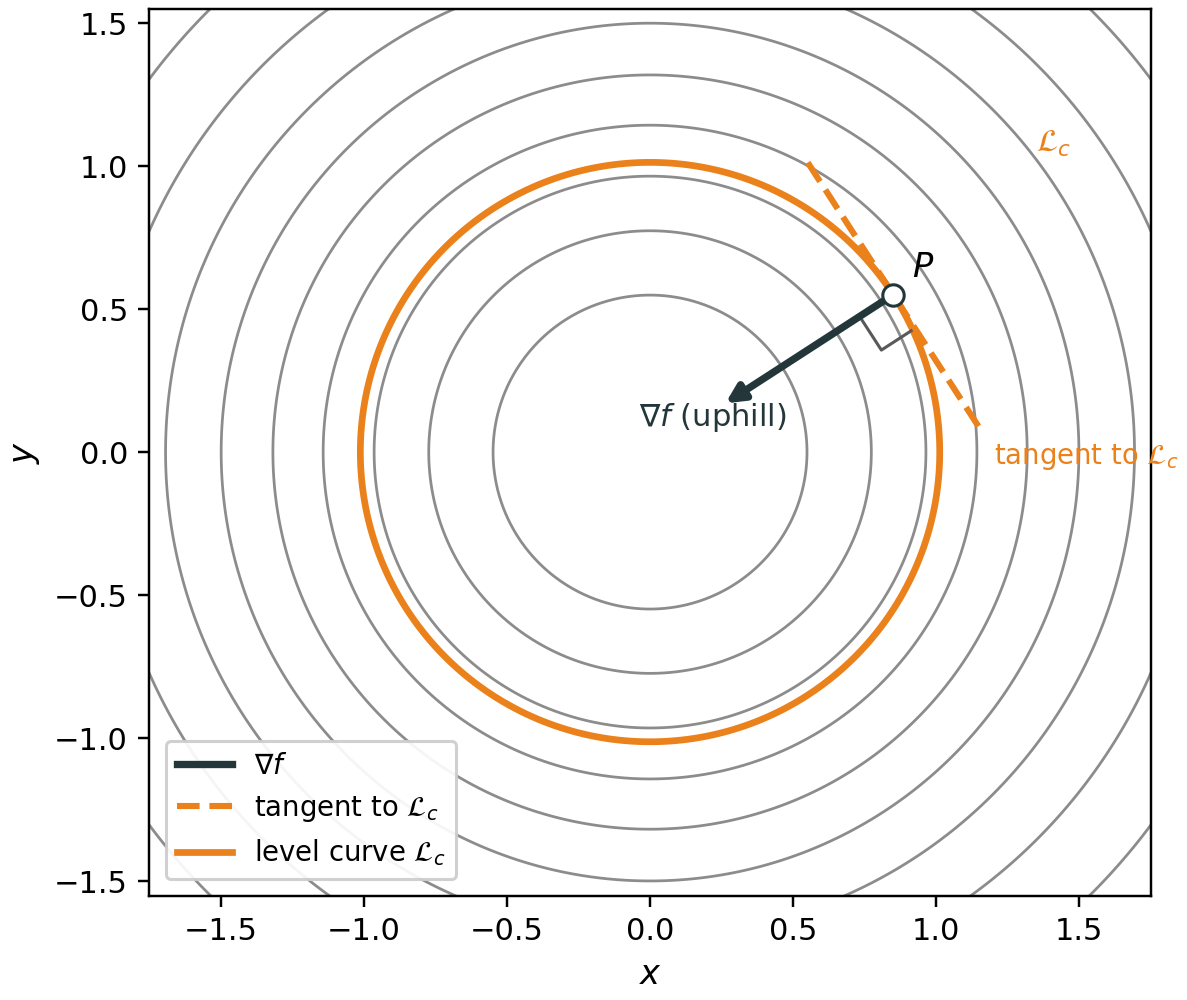
\includegraphics[width=0.98\linewidth]{figures/gradient_contour.png}
  \end{columns}
\end{frame}

\begin{frame}{1.8 Directional derivative}
  \footnotesize
  \textbf{Definition.}\ For unit direction $\mathbf{u}=(u_1,u_2)$,
  $\|\mathbf{u}\|=1$, the \textbf{directional derivative} at $(a,b)$ is
  \[
    D_{\mathbf{u}}f(a,b)
    :=\lim_{t\to 0}\frac{f(a+tu_1,\,b+tu_2)-f(a,b)}{t}
  \]
  (rate of change of $f$ per unit step along $\mathbf{u}$).

  \medskip
  \textbf{Derive.}\ Step $(dx,dy)=t\mathbf{u}$. By the total differential,
  for small $t$,
  \[
    f(a+tu_1,b+tu_2)-f(a,b)
    \approx f_x(tu_1)+f_y(tu_2)
    =t\,\nabla f\cdot\mathbf{u}.
  \]
  Divide by $t$ and let $t\to 0$:
  \[
    D_{\mathbf{u}}f(a,b)=\nabla f\cdot\mathbf{u}
    =\|\nabla f\|\cos\theta.
  \]
\end{frame}

\begin{frame}{1.8 Example: targeted input change --- question}
  \footnotesize
  \textbf{A firm's output with a targeted input change.}

  \medskip
  Cobb--Douglas production (capital $K$, labor $L$):
  \[
    Q(K,L)=K^{\alpha}L^{1-\alpha},\qquad \alpha=0.5.
  \]
  Current inputs: $(K_0,L_0)=(100,100)$.

  \medskip
  A subsidy is paid only if the firm increases \textbf{both} inputs in ratio
  $2{:}1$ (for every 1 unit of labor, add 2 units of capital).

  \medskip
  This defines direction $\mathbf{v}=(2,1)$ in $(K,L)$-space.

  \medskip
  \textbf{Question:}\ How fast does output $Q$ change per unit step in that
  direction?
\end{frame}

\begin{frame}{1.8 Example: targeted input change --- solution}
  \footnotesize
  \textbf{1.\ Gradient at $(100,100)$.}
  $Q_K=0.5K^{-0.5}L^{0.5}$,\ $Q_L=0.5K^{0.5}L^{-0.5}$.
  Since $100^{0.5}=10$ and $100^{-0.5}=0.1$,
  \[
    Q_K=0.5(0.1)(10)=0.5,\qquad Q_L=0.5(10)(0.1)=0.5.
  \]
  So $\nabla Q=(0.5,\,0.5)$.

  \medskip
  \textbf{2.\ Unit direction.}\ $\|\mathbf{v}\|=\sqrt{5}$,
  \[
    \mathbf{u}=\Bigl(\tfrac{2}{\sqrt{5}},\,\tfrac{1}{\sqrt{5}}\Bigr).
  \]

  \medskip
  \textbf{3.\ Directional derivative.}
  \[
    D_{\mathbf{u}}Q=\nabla Q\cdot\mathbf{u}
    =0.5\Bigl(\tfrac{2}{\sqrt{5}}+\tfrac{1}{\sqrt{5}}\Bigr)
    =\frac{1.5}{\sqrt{5}}\approx 0.67.
  \]

  \medskip
  {\scriptsize \textbf{Interpretation:}\ from $(100,100)$, moving in direction
  $\mathbf{u}$ (ratio $2{:}1$), output rises at initial rate
  $\approx 0.67$ units of $Q$ per unit distance in input space.}
\end{frame}

\begin{frame}{1.8 Cross-partial derivatives and Schwarz}
  \footnotesize
  \textbf{Cross-partials.}\ For $f(x,y)$,
  \[
    f_{xy}=\frac{\partial^2 f}{\partial x\,\partial y}
    =\frac{\partial}{\partial x}\!\left(\frac{\partial f}{\partial y}\right),
    \qquad
    f_{yx}=\frac{\partial^2 f}{\partial y\,\partial x}
    =\frac{\partial}{\partial y}\!\left(\frac{\partial f}{\partial x}\right).
  \]

  \medskip
  \textbf{Schwarz's theorem (stated).}\ If $f_{xy}$ and $f_{yx}$ exist and are
  continuous near $(a,b)$, then $f_{xy}(a,b)=f_{yx}(a,b)$.

  \medskip
  \textbf{Example.}\ $Y=K^{\alpha}L^{1-\alpha}$:
  \[
    \frac{\partial MP_K}{\partial L}
    =Y_{KL}=\alpha(1-\alpha)K^{\alpha-1}L^{-\alpha}
    =\frac{\partial MP_L}{\partial K}=Y_{LK}.
  \]

  \medskip
  {\scriptsize \textbf{Econ:}\ $Y_{KL}$ tells how $MP_K$ changes when $L$ rises
  (and vice versa). Sign of $Y_{KL}$: complements ($+$) vs.\ substitutes ($-$).}
\end{frame}

\section{1.9 --- Limits}

\begin{frame}{1.9 Limits --- why this section}
  \footnotesize
  \textbf{Berkeley's critique (1734).}\ Early calculus treated $h$ as
  ``infinitely small'': nonzero when dividing, then set to $0$.
  Berkeley called these \textbf{``ghosts of departed quantities''} --- logically
  suspicious.

  \medskip
  \textbf{Example:}\ $f(x)=x^2$ at $a=3$.
  \[
    \frac{f(3+h)-f(3)}{h}
    =\frac{(3+h)^2-9}{h}
    =\frac{6h+h^2}{h}
    =6+h\qquad(h\neq 0).
  \]
  Early calculus: ``let $h\to 0$'' to get $f'(3)=6$.

  \medskip
  \textbf{Berkeley's objection.}\ The algebra \textbf{requires} $h\neq 0$ to divide by
  $h$; then we act as if $h=0$ at the end.
  That is the ghost: $h$ is treated as both present and absent.
\end{frame}

\begin{frame}{1.9 Limit of a sequence ($\varepsilon$-$N$)}
  \footnotesize
  Let $(a_n)$ be a sequence and $L\in\mathbb{R}$.

  \medskip
  \textbf{Definition.}\ $\displaystyle\lim_{n\to\infty}a_n=L$ means:
  \[
    \forall\,\varepsilon>0\;\;\exists\,N\in\mathbb{N}\;\;\forall\,n\ge N:\quad
    |a_n-L|<\varepsilon.
  \]

  \medskip
  \textbf{Reading the quantifiers.}
  \begin{itemize}\itemsep2pt
    \item $\varepsilon$: target accuracy (how close to $L$ you want).
    \item $N$: step after which the sequence stays inside that accuracy.
    \item Order matters: you choose $\varepsilon$ first, \emph{then} find $N$.
  \end{itemize}

  \medskip
  {\scriptsize If the limit exists, the sequence \textbf{converges} to $L$;
  otherwise it \textbf{diverges}.}
\end{frame}

\begin{frame}{1.9 Limit of a function ($\varepsilon$-$\delta$)}
  \footnotesize
  $\displaystyle\lim_{x\to a}f(x)=L$ means
  {\scriptsize$\forall\,\varepsilon>0\;\exists\,\delta>0\;\forall\,x\in D$:
  $0<|x-a|<\delta\Rightarrow|f(x)-L|<\varepsilon$.}

  \medskip
  \begin{columns}[T,onlytextwidth]
    \column{0.48\textwidth}
    \vspace{0.25cm}
    \textbf{Example.}\ $f(x)=x+1$ for $x\neq 1$;\ $f(1)=3$.

    \medskip
    \[
      \lim_{x\to 1}f(x)=2,
      \qquad
      f(1)=3\neq 2.
    \]

    \medskip
    For $\varepsilon=\tfrac12$, take $\delta=\tfrac12$.

    \medskip
    If $0<|x-1|<\delta$, then
    \[
      |f(x)-2|=|x-1|<\varepsilon.
    \]

    \column{0.50\textwidth}
    \centering
    \vspace{-0.15cm}
    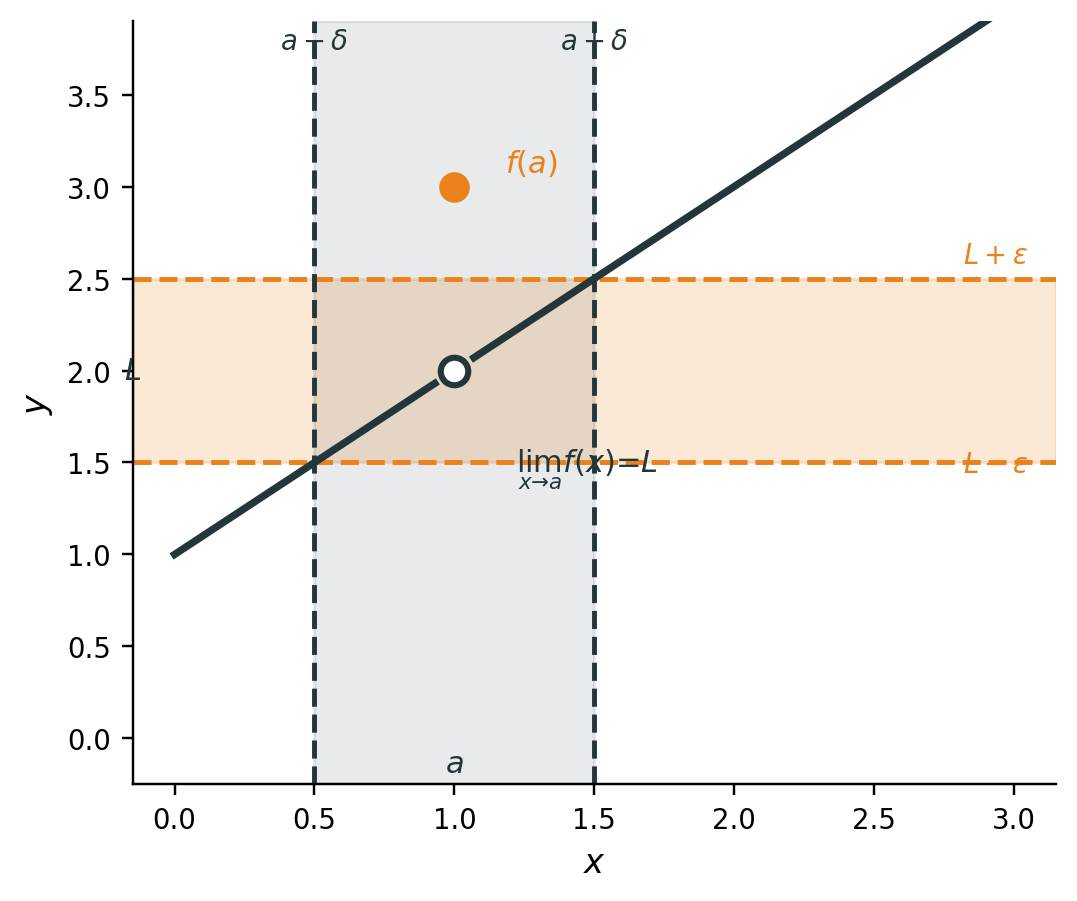
\includegraphics[width=\linewidth]{figures/epsilon_delta_limit.png}

    \vspace{2pt}
    {\scriptsize On $0<|x-a|<\delta$, the curve stays in the $\varepsilon$-band
    around $L$; the value at $x=a$ is ignored.}
  \end{columns}
\end{frame}

\begin{frame}{1.9 Continuous and differentiable}
  \footnotesize
  \textbf{Continuous at $a$.}\ $f$ is continuous at $a$ if
  \[
    \lim_{x\to a}f(x)=f(a).
  \]
  So the limit exists \textbf{and} equals the function value at $a$.

  \medskip
  \textbf{Differentiable at $a$.}\ $f$ is differentiable at $a$ if
  \[
    f'(a)=\lim_{h\to 0}\frac{f(a+h)-f(a)}{h}
  \]
  exists (finite).

  \medskip
  \textbf{Relation.}\ Differentiable at $a$ $\Rightarrow$ continuous at $a$.
  {\scriptsize Converse fails: see examples on the next slide.}
\end{frame}

\begin{frame}{1.9 Continuous but not differentiable --- for interest}
  \scriptsize
  \begin{columns}[T,onlytextwidth]
    \column{0.48\textwidth}
    \centering
    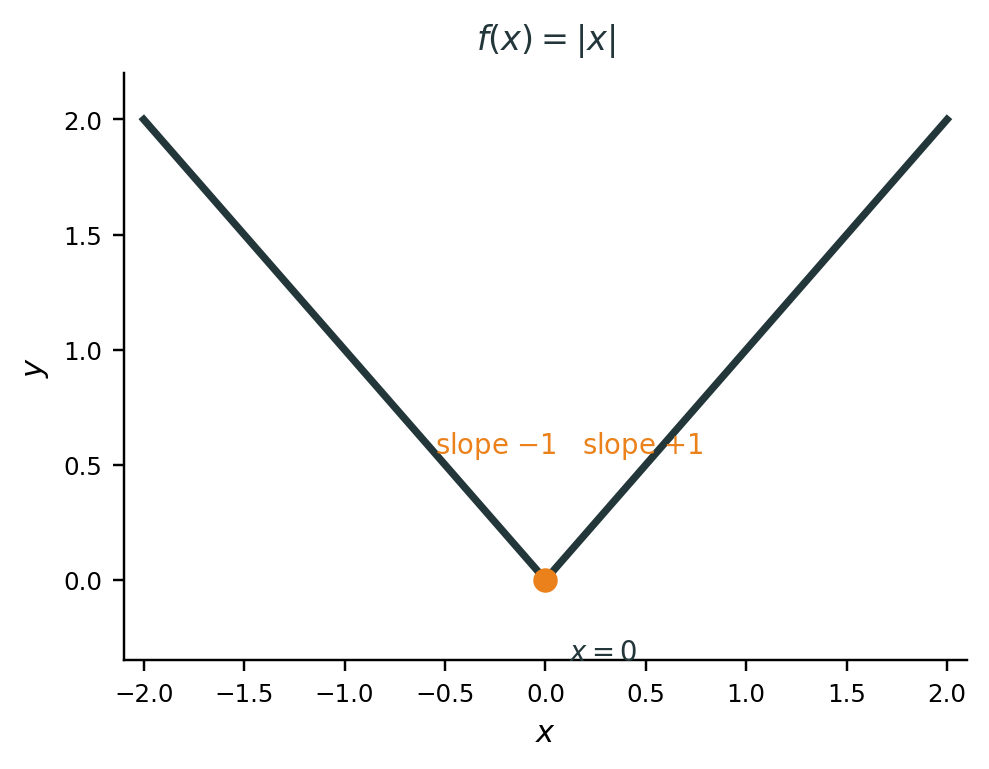
\includegraphics[width=0.92\linewidth]{figures/abs_x_corner.png}

    \textbf{$f(x)=|x|$.}\ Continuous on $\mathbb{R}$; at $0$,
    left slope $-1$ and right slope $+1$ disagree
    $\Rightarrow$ not differentiable at $0$.

    \column{0.48\textwidth}
    \centering
    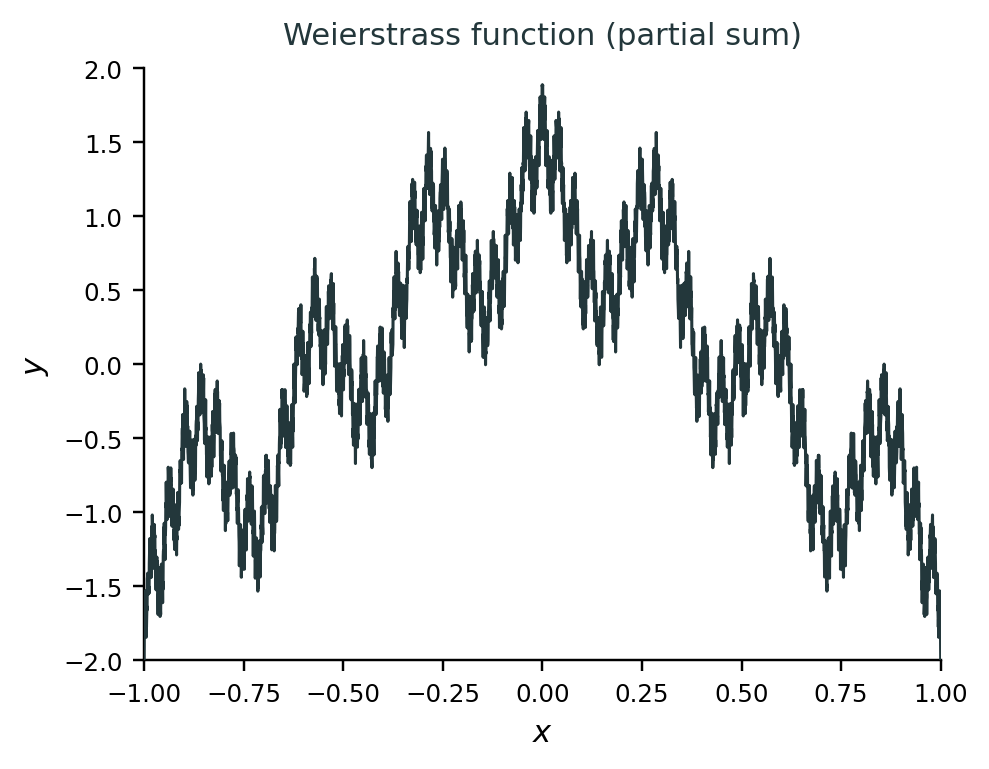
\includegraphics[width=0.92\linewidth]{figures/weierstrass_partial.png}

    \textbf{Weierstrass (1872).}\ Some $W\colon\mathbb{R}\to\mathbb{R}$ is
    \textbf{continuous everywhere} but \textbf{differentiable nowhere}.
    {\scriptsize Plot: $10$ terms of
    $\sum_{n=0}^{\infty}a^n\cos(b^n\pi x)$, $a=\tfrac12$, $b=7$.}
  \end{columns}
\end{frame}

\begin{frame}{1.9 Multivariable: continuous and differentiable}
  \footnotesize
  For $f\colon\mathbb{R}^n\to\mathbb{R}$, write $\mathbf{a}\in\mathbb{R}^n$,
  $\mathbf{h}\in\mathbb{R}^n$ with $\|\mathbf{h}\|=\sqrt{h_1^2+\cdots+h_n^2}$.

  \medskip
  \textbf{Continuous at $\mathbf{a}$.}
  \[
    \lim_{\mathbf{x}\to\mathbf{a}} f(\mathbf{x}) = f(\mathbf{a}).
  \]

  \medskip
  {\scriptsize Must hold as $\mathbf{x}\to\mathbf{a}$ along \textbf{every path}
  (every direction). If two paths give different limits, $f$ is not continuous at
  $\mathbf{a}$.}

  \medskip
  \textbf{Differentiable at $\mathbf{a}$.}\ There is a vector
  $\nabla f(\mathbf{a})=(f_{x_1}(\mathbf{a}),\ldots,f_{x_n}(\mathbf{a}))$ such that
  \[
    f(\mathbf{a}+\mathbf{h})
    = f(\mathbf{a}) + \nabla f(\mathbf{a})\cdot\mathbf{h} + r(\mathbf{h}),
    \qquad
    \frac{r(\mathbf{h})}{\|\mathbf{h}\|}\to 0 \ \text{as}\ \mathbf{h}\to\mathbf{0}.
  \]

  \medskip
  \textbf{Tangent plane (two variables).}\ If $f(x,y)$ is differentiable at $(a,b)$,
  the graph $z=f(x,y)$ has a tangent plane at $(a,b,f(a,b))$:
  \[
    z - f(a,b) = f_x(a,b)(x-a) + f_y(a,b)(y-b).
  \]
  {\scriptsize The linear term $\nabla f(a,b)\cdot\mathbf{h}$ is exactly this plane:
  the best linear approximation to $f$ near $(a,b)$.}
\end{frame}

\begin{frame}{1.9 Differentiable $\Rightarrow$ continuous}
  \footnotesize
  \textbf{Proposition.}\ If $f\colon\mathbb{R}^n\to\mathbb{R}$ is differentiable at
  $\mathbf{a}$, then $f$ is continuous at $\mathbf{a}$.

  \medskip
  \textbf{Proof.}\ Write $\mathbf{h}=\mathbf{x}-\mathbf{a}$. By differentiability,
  \[
    f(\mathbf{x})-f(\mathbf{a})
    = \nabla f(\mathbf{a})\cdot\mathbf{h} + r(\mathbf{h}).
  \]
  As $\mathbf{x}\to\mathbf{a}$, we have $\mathbf{h}\to\mathbf{0}$, so
  $\nabla f(\mathbf{a})\cdot\mathbf{h}\to 0$ and $r(\mathbf{h})\to 0$.
  Hence $f(\mathbf{x})\to f(\mathbf{a})$.
  \hfill$\square$
\end{frame}

\begin{frame}{1.9 Example: differentiable in two variables}
  \footnotesize
  \textbf{Example.}\ $f(x,y)=x^2+y^2$ is differentiable at every $(a,b)$.

  \medskip
  \textbf{Check at $(a,b)$.}\ Expand:
  \[
    f(a+h,b+k)-f(a,b)
    = (a+h)^2+(b+k)^2-(a^2+b^2)
    = 2ah+2bk + (h^2+k^2).
  \]
  Here $\nabla f(a,b)=(2a,2b)$ and the linear part is $2ah+2bk$.
  The remainder is $r(h,k)=h^2+k^2$, and
  \[
    \frac{|r(h,k)|}{\|(h,k)\|}
    = \frac{h^2+k^2}{\sqrt{h^2+k^2}}
    = \sqrt{h^2+k^2}\to 0.
  \]
  So $f$ is differentiable at $(a,b)$ with $df=2a\,dx+2b\,dy$.

  \medskip
  {\scriptsize By the proposition on the previous slide, $f$ is also continuous at $(a,b)$.}
\end{frame}

\begin{frame}{1.9 Partials exist $\not\Rightarrow$ differentiable --- for interest}
  \footnotesize
  \begin{columns}[T,onlytextwidth]
    \column{0.46\textwidth}
    Partials at $(a,b)$ alone do \textbf{not} imply differentiable, and do
    \textbf{not} imply a tangent plane exists.

    \medskip
    \textbf{Example.}\ Define
    \[
      f(x,y)=
      \begin{cases}
        \dfrac{xy}{x^2+y^2}, & (x,y)\neq(0,0),\\[4pt]
        0, & (x,y)=(0,0).
      \end{cases}
    \]
    \textbf{Partials at $(0,0)$:}\ $f(x,0)=0$, $f(0,y)=0$
    $\Rightarrow$ $f_x(0,0)=f_y(0,0)=0$.

    \medskip
    \textbf{But not continuous at $(0,0)$:}\
    along $y=x$, $f(x,x)=\tfrac12$ for $x\neq 0$;
    along $y=0$, $f=0$.
    Different paths, different limits.

    \medskip
    {\scriptsize So no tangent plane: the graph cannot be approximated by one plane
    from every direction.}

    \column{0.52\textwidth}
    \centering
    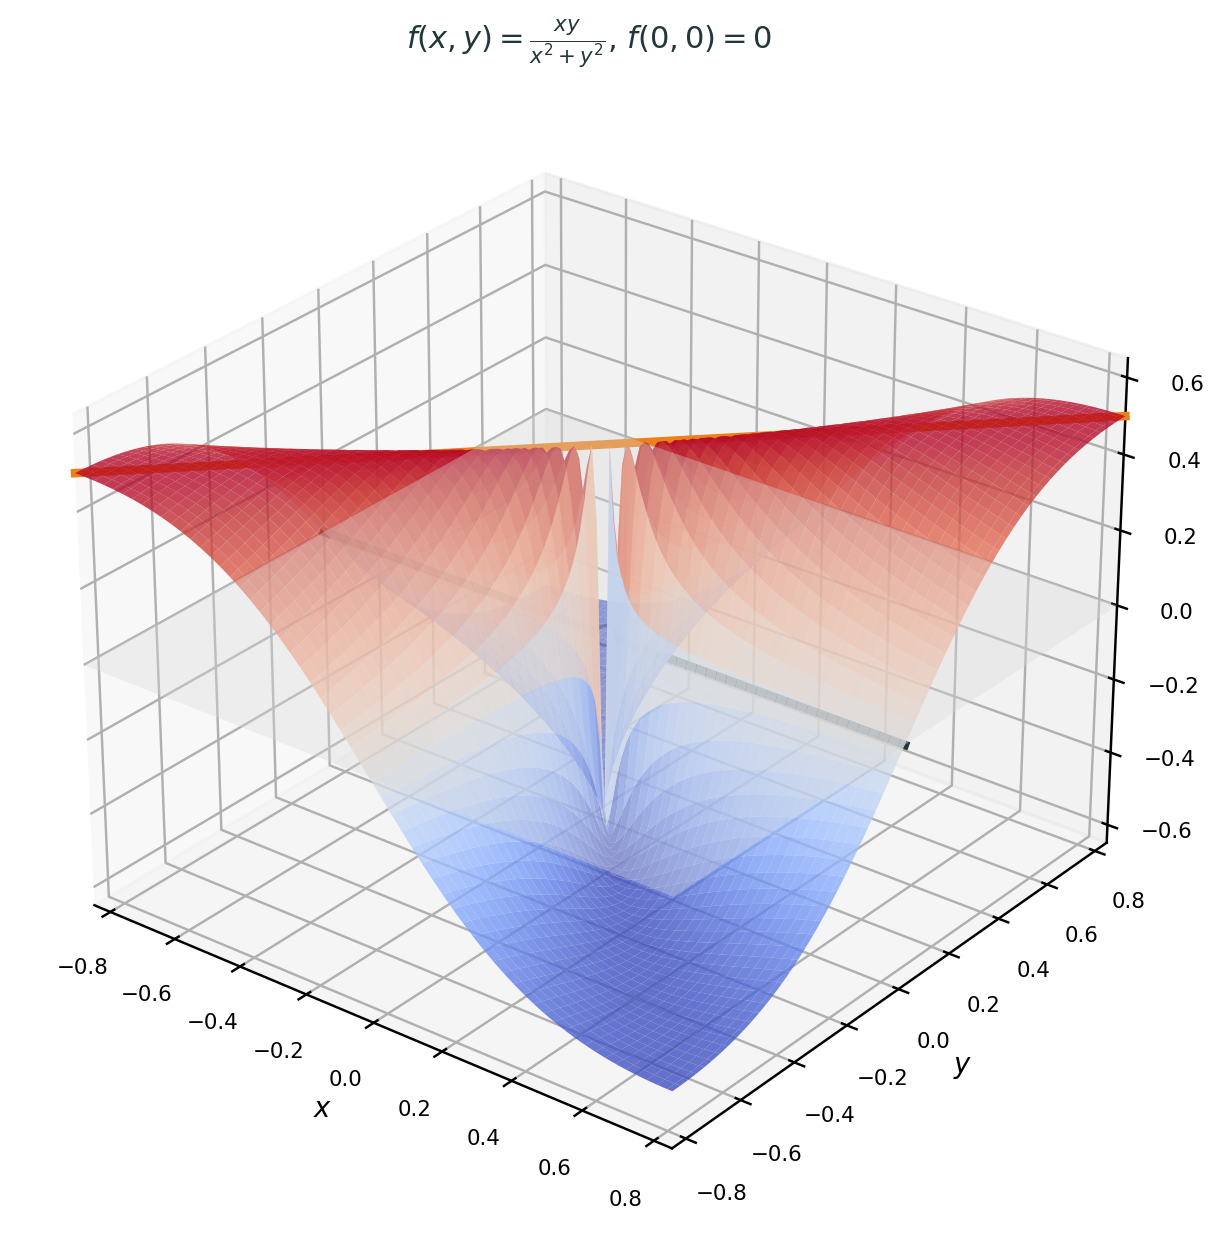
\includegraphics[width=\linewidth]{figures/partials_not_differentiable.png}
  \end{columns}
\end{frame}

\QFrame{1.9 --- Limits practice}
  \footnotesize
  \textbf{Practice.}

  \vspace{4pt}
  \onslide<2->{\textbf{1.}\ Let $f(x)=x^2$.
    Use $\varepsilon$-$\delta$ to prove $f'(a)=2a$.\par}
  \onslide<3->{\textbf{Goal.}\ $\forall\,\varepsilon>0\;\exists\,\delta>0$:\ if
    $0<|h|<\delta$, then
    $\bigl|\frac{f(a+h)-f(a)}{h}-2a\bigr|<\varepsilon$.\par}
  \onslide<4->{\textbf{Algebra.}\ For $h\neq 0$,
    $\displaystyle\frac{(a+h)^2-a^2}{h}
    =\frac{2ah+h^2}{h}=2a+h$.\par}
  \onslide<5->{\textcolor{mAccent}{\textbf{Choose $\delta=\varepsilon$.}\ Then
    $\bigl|\frac{f(a+h)-f(a)}{h}-2a\bigr|=|h|<\varepsilon$.}\hfill
    {\scriptsize so $f'(a)=2a$}}\par\medskip

  \onslide<6->{\textbf{2.}\ $f(x)=x+1$ for $x\neq 1$;\ $f(1)=3$.
    Use $\varepsilon$-$\delta$ to prove $\displaystyle\lim_{x\to 1}f(x)=2$.\par}
  \onslide<7->{\textbf{Goal.}\ $\forall\,\varepsilon>0\;\exists\,\delta>0$:\ if
    $0<|x-1|<\delta$, then $|f(x)-2|<\varepsilon$.\par}
  \onslide<8->{\textbf{Algebra.}\ For $x\neq 1$ near $1$, $f(x)=x+1$, so
    $|f(x)-2|=|x-1|$.\par}
  \onslide<9->{\textcolor{mAccent}{\textbf{Choose $\delta=\varepsilon$.}\ Then
    $|f(x)-2|=|x-1|<\varepsilon$.}\hfill
    {\scriptsize $f(1)=3\neq 2$: limit exists, but $f$ not continuous at $1$}}\par
\end{frame}

\appendix

\section{Single-variable derivative rules --- derivations}

\begin{frame}{A.1 Deriving rules (I): constants, sums, powers}
  \small
  Write $D_a f=f'(a)=\displaystyle\lim_{h\to 0}\frac{f(a+h)-f(a)}{h}$.

  \medskip
  \textbf{Constant:}\ $f(x)=c$ $\Rightarrow$
  $D_a f=\displaystyle\lim_{h\to 0}\frac{c-c}{h}=0$.

  \medskip
  \textbf{Sum:}\ $D_a(f+g)=D_a f+D_a g$
  (split the numerator; limits add).

  \medskip
  \textbf{Power rule} (integer $n\ge 1$):\ for $f(x)=x^n$,
  \[
    \frac{(a+h)^n-a^n}{h}
    =\frac{a^n+na^{n-1}h+\cdots+h^n-a^n}{h}
    =na^{n-1}+\text{terms with extra factors of }h
    \;\xrightarrow[h\to 0]{}\; na^{n-1}.
  \]
  So $(x^n)'=nx^{n-1}$.
\end{frame}

\begin{frame}{A.2 Deriving rules (II): product and quotient}
  \small
  \textbf{Product rule.}\ For $h(x)=f(x)g(x)$,
  \[
    \frac{h(a+h)-h(a)}{h}
    =f(a+h)\frac{g(a+h)-g(a)}{h}
     +g(a)\frac{f(a+h)-f(a)}{h}
     \;\xrightarrow[h\to 0]{}\;
     f(a)g'(a)+f'(a)g(a).
  \]
  So $(fg)'=f'g+fg'$.

  \medskip
  \textbf{Quotient rule.}\ Write $\dfrac{f}{g}=f\cdot g^{-1}$.
  For $y=1/g$, $\ln y=-\ln g$, so
  $\dfrac{y'}{y}=-\dfrac{g'}{g}\Rightarrow y'=-\dfrac{g'}{g^2}$.
  Then product rule gives
  $\Bigl(\dfrac{f}{g}\Bigr)'=\dfrac{f'g-fg'}{g^2}$.
\end{frame}

\begin{frame}{A.3 Key facts for exp and log}
  \footnotesize
  \textbf{Fact 1:}\ $\displaystyle\lim_{h\to 0}\frac{e^h-1}{h}=1$.

  \smallskip
  \textbf{Why?}\ Start with
  $e=\displaystyle\lim_{n\to\infty}\Bigl(1+\tfrac{1}{n}\Bigr)^n$ and
  $e^x=\displaystyle\lim_{n\to\infty}\Bigl(1+\tfrac{x}{n}\Bigr)^n$.
  Binomial expansion:
  \[
    \Bigl(1+\tfrac{h}{n}\Bigr)^n
    =1+h+\frac{n(n-1)}{2n^2}h^2+\cdots
    \;\xrightarrow[n\to\infty]{}\; e^h.
  \]
  So $e^h=1+h+O(h^2)$, hence
  $\dfrac{e^h-1}{h}=1+O(h)\to 1$.

  \medskip
  \textbf{Fact 2:}\ $\displaystyle\lim_{u\to 0}\frac{\ln(1+u)}{u}=1$.

  \smallskip
  \textbf{Why?}\ For small $u$, Fact~1 gives $e^u\approx 1+u$.
  If $v=\ln(1+u)$, then $e^v=1+u$, so $v\approx u$ and
  $\dfrac{\ln(1+u)}{u}\approx 1$.
  Equivalently, Taylor: $\ln(1+u)=u-\tfrac{u^2}{2}+\cdots$.
\end{frame}

\begin{frame}{A.4 Deriving the exponential: $(e^x)'=e^x$}
  \small
  Use Fact~1 from the previous slide:
  $\displaystyle\lim_{h\to 0}\frac{e^h-1}{h}=1$.

  \medskip
  For $f(x)=e^x$,
  \[
    f'(a)=\lim_{h\to 0}\frac{e^{a+h}-e^a}{h}
    =e^a\lim_{h\to 0}\frac{e^h-1}{h}
    =e^a.
  \]
  So $(e^x)'=e^x$.

  \medskip
  {\scriptsize Reading: a small step $h$ multiplies $e^x$ by about $1+h$.}
\end{frame}

\begin{frame}{A.5 Deriving the logarithm: $(\ln x)'=\tfrac{1}{x}$}
  \small
  \textbf{Method 1 (inverse function).}\ If $y=\ln x$, then $e^y=x$.
  Differentiate: $e^y\,y'=1$, so $y'=\dfrac{1}{e^y}=\dfrac{1}{x}$.

  \medskip
  \textbf{Method 2 (limit definition).}\ For $a>0$, set $u=h/a$:
  \[
    \frac{\ln(a+h)-\ln a}{h}
    =\frac{1}{h}\ln\!\Bigl(1+\frac{h}{a}\Bigr)
    =\frac{1}{a}\cdot\frac{\ln(1+u)}{u}
    \;\xrightarrow[u\to 0]{}\;
    \frac{1}{a},
  \]
  by Fact~2. So $(\ln x)'=\tfrac{1}{x}$.
\end{frame}

\end{document}
